\documentclass[11pt,french,a4paper]{article}
\usepackage[utf8]{inputenc}
\usepackage[french]{babel}
\usepackage[T1]{fontenc}
\usepackage{fancyhdr}
\usepackage{lastpage}
\usepackage{fancybox}
\usepackage{graphicx}
\usepackage{appendix}
\usepackage[left=2cm,right=2cm,top=2cm,bottom=2.5cm]{geometry}
\geometry{a4paper}
\setlength{\parindent}{0pt}
\usepackage{listings}
\usepackage{color}
\usepackage[table]{xcolor}
\usepackage{array}
\usepackage{listings}
\usepackage{hyperref}
\usepackage{caption}
\usepackage{lastpage}
\pagestyle{fancy}

\definecolor{darkWhite}{rgb}{0.94,0.94,0.94}

\lstset{
  aboveskip=3mm,
  belowskip=-2mm,
  backgroundcolor=\color{darkWhite},
  basicstyle=\footnotesize,
  breakatwhitespace=false,
  breaklines=true,
  captionpos=b,
  commentstyle=\color{red},
  deletekeywords={...},
  escapeinside={\%*}{*)},
  extendedchars=true,
  framexleftmargin=16pt,
  framextopmargin=3pt,
  framexbottommargin=6pt,
  frame=tb,
  keepspaces=true,
  keywordstyle=\color{blue},
  language=C,
  literate=
  {²}{{\textsuperscript{2}}}1
  {⁴}{{\textsuperscript{4}}}1
  {⁶}{{\textsuperscript{6}}}1
  {⁸}{{\textsuperscript{8}}}1
  {€}{{\euro{}}}1
  {é}{{\'e}}1
  {è}{{\`{e}}}1
  {ê}{{\^{e}}}1
  {ë}{{\¨{e}}}1
  {É}{{\'{E}}}1
  {Ê}{{\^{E}}}1
  {û}{{\^{u}}}1
  {ù}{{\`{u}}}1
  {â}{{\^{a}}}1
  {à}{{\`{a}}}1
  {á}{{\'{a}}}1
  {ã}{{\~{a}}}1
  {Á}{{\'{A}}}1
  {Â}{{\^{A}}}1
  {Ã}{{\~{A}}}1
  {ç}{{\c{c}}}1
  {Ç}{{\c{C}}}1
  {õ}{{\~{o}}}1
  {ó}{{\'{o}}}1
  {ô}{{\^{o}}}1
  {Õ}{{\~{O}}}1
  {Ó}{{\'{O}}}1
  {Ô}{{\^{O}}}1
  {î}{{\^{i}}}1
  {Î}{{\^{I}}}1
  {í}{{\'{i}}}1
  {Í}{{\~{Í}}}1,
  morekeywords={*,...},
  numbers=left,
  numbersep=10pt,
  numberstyle=\tiny\color{black},
  rulecolor=\color{black},
  showspaces=false,
  showstringspaces=false,
  showtabs=false,
  stepnumber=1,
  stringstyle=\color{gray},
  tabsize=4,
  title=\lstname,
}

\fancyhead[L]{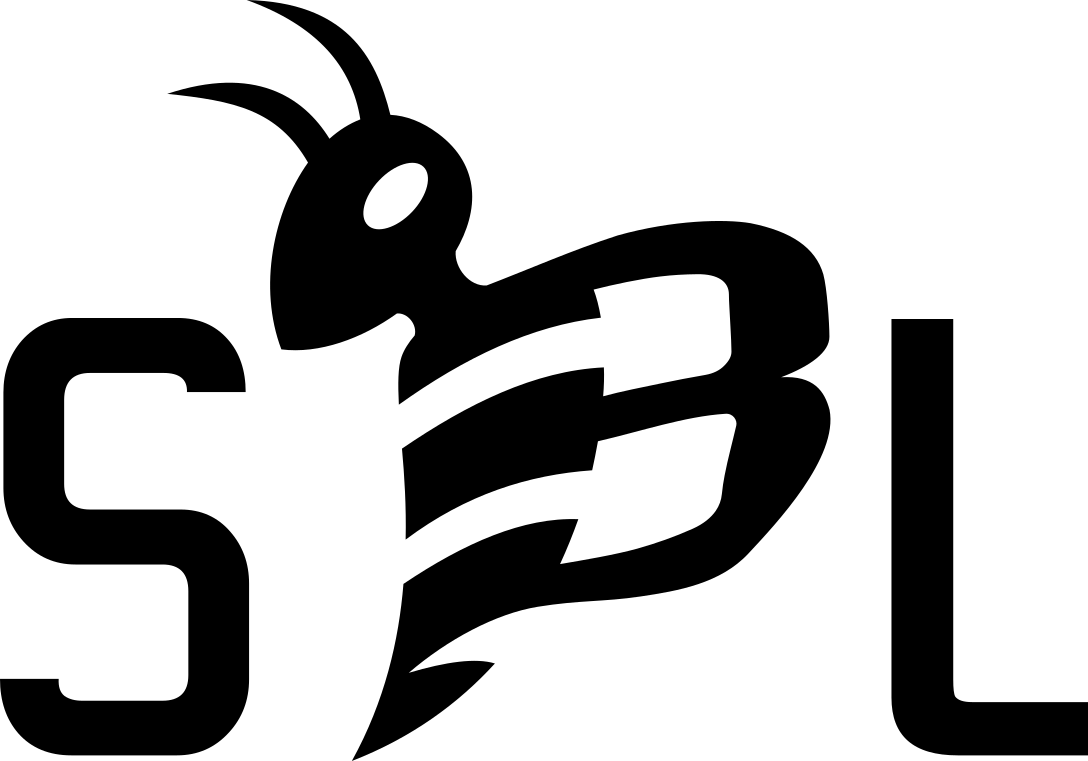
\includegraphics[width=1cm]{../../../logo/SBLlogo.png}}
\fancyhead[C]{Rapport d'activités mois de mai 2022 }
\fancyhead[R]{ 
\includegraphics[width=1.2cm]{../../../logo/IUTlogo.png}}
\fancyfoot[L]{\small Tom TUELEAU\normalsize}
\fancyfoot[C]{}
\fancyfoot[R]{\thepage/\pageref{LastPage}}

\lstset{
  basicstyle=\fontfamily{lmvtt}\selectfont\small,
  columns=fullflexible,
}

\title{
	\bigskip
 \centering
         
\includegraphics[width=4cm]{../../../logo/IUTlogo.png}  \hspace{7cm}
         
\includegraphics[width=4cm]{../../../logo/UMlogo.png}  \hspace{7cm}

	\LARGE{Rapport de stage}
	\\
	\LARGE{IBMM}
	\\
	\large{\textbf{Institut des Biomolécules Max Mousseron}}
	\\
	\large{Stagiaire :\textbf{Tom TUELEAU}}
	\\
	\large{Tuteur de stage :\textbf{Matthieu ROUSSET}}
	\\
	\large{Tuteur académique :\textbf{Sébastien DRUON}}
	\\
	\large{RT2 :Promotion 2020-2022}
	\\
         
\includegraphics[width=4cm]{../../../logo/LIRMMlogo.png}  \hspace{7cm}
         \includegraphics[width=4cm]{../../../logo/IBMMlogo.jpg}  \hspace{7cm}
}
\author{
	\date{}
}

\begin{document}

\maketitle

\newpage
\section*{Remerciment}
J’adresse mes sincères remerciements aux personnes qui m’ont permis de réaliser ce stage.
Je souhaite remercier M. Matthieu Rousset, initiateur du projet SuperBeeLive,de m’avoir accepté au sein de son équipe.
Je souhaite également remercier Mme Olivia Serenelli-Pesin, qui a su m’encadrer et me guider. tout au long de ce stage
Je remercie également M. Sebastien Druon pour m’avoir conseiller et aiguillier quand j'ai rencontrées des difficulter lors de mes mission.
Et enfin je remercie vivement toute l’équipe de pédagogique de Béziers, qui a su m'enseigmer le savoir utile lors de ce stage.

\newpage
\tableofcontents

\newpage
\section{Introduction}
Ce rapport feras états de l'activiter réalisée lors du stage ainsi que l'états d'avancement des differentes missions confier. Ma missions principal était la suivante : (Extrait de "sujets\_stage\_tom" de Mme Olivia SERENELLI-PESIN) 
\\
\\
\fbox{
	\begin{minipage}{17cm} 
	Nous avons besoin de mettre en place une première installation avec un micro-controleur et des capteurs dans la ruche afin de faire un "proof of concept" simple pour pouvoir afficher les données enregistrée sur le site internet où les vidéos des abeilles seront diffusées.\\
	\\
	Les données à enregistrer seront :\\
	— Température\\
	— Hygrométrie\\
	— Capteur de vibration fixé sur une gaufre de la ruche\\
	\\
	Elles devront être remontées en MQTT sur un serveur déjà mis en place.
	Le tout doit être opérationnel (fonctionnel et dans la ruche) avant le 15 Mai 2022.
	\\
	\end{minipage}
}
\\
\\
Je commencerait donc par vous présenter l'environement dans le quel j'ai travailler. Une seconde partie décrira la maniére dont je me suis organiser. Je décrirait aussi le réseau sur le qu'elle j'ai travailler, ainsi que les choix fait quand aux protocoles utiliser. Une quatrième partie aborderas les montages éléctronique que j'ai découvert et testés lors de ce stage. Une dernier partie abordera la programmation des différent composant du système. Enfin, je conclurait en abordant les probléme rencontrer ainsi que les amélioration à effectuer pour le stage.

\newpage
\section{Infrastructure}
\subsection{Mise en situation}
Mon stage prend place dans le projet SuperBeeLive 

J'ai passer la majoriter de mon stage au rucher, lieu ou sont entreposer une dizaine de ruche et ou la majoriter du projet SuperBeeLive prend place.
Nous étions plusieur stagiaire installer à cet endroit. J'ai donc pu colaborer avec plusieurs d'entre eux notament sur la redaction de nos rappeur. Comme vous pouvez le voire sur les figures \ref{Intérieur du rucher} et \ref{Extérieur du rucher}  nous étions installé dans un préfabriqué (climatiser et fibrer) situer à coter des ruches.

\begin{center}	
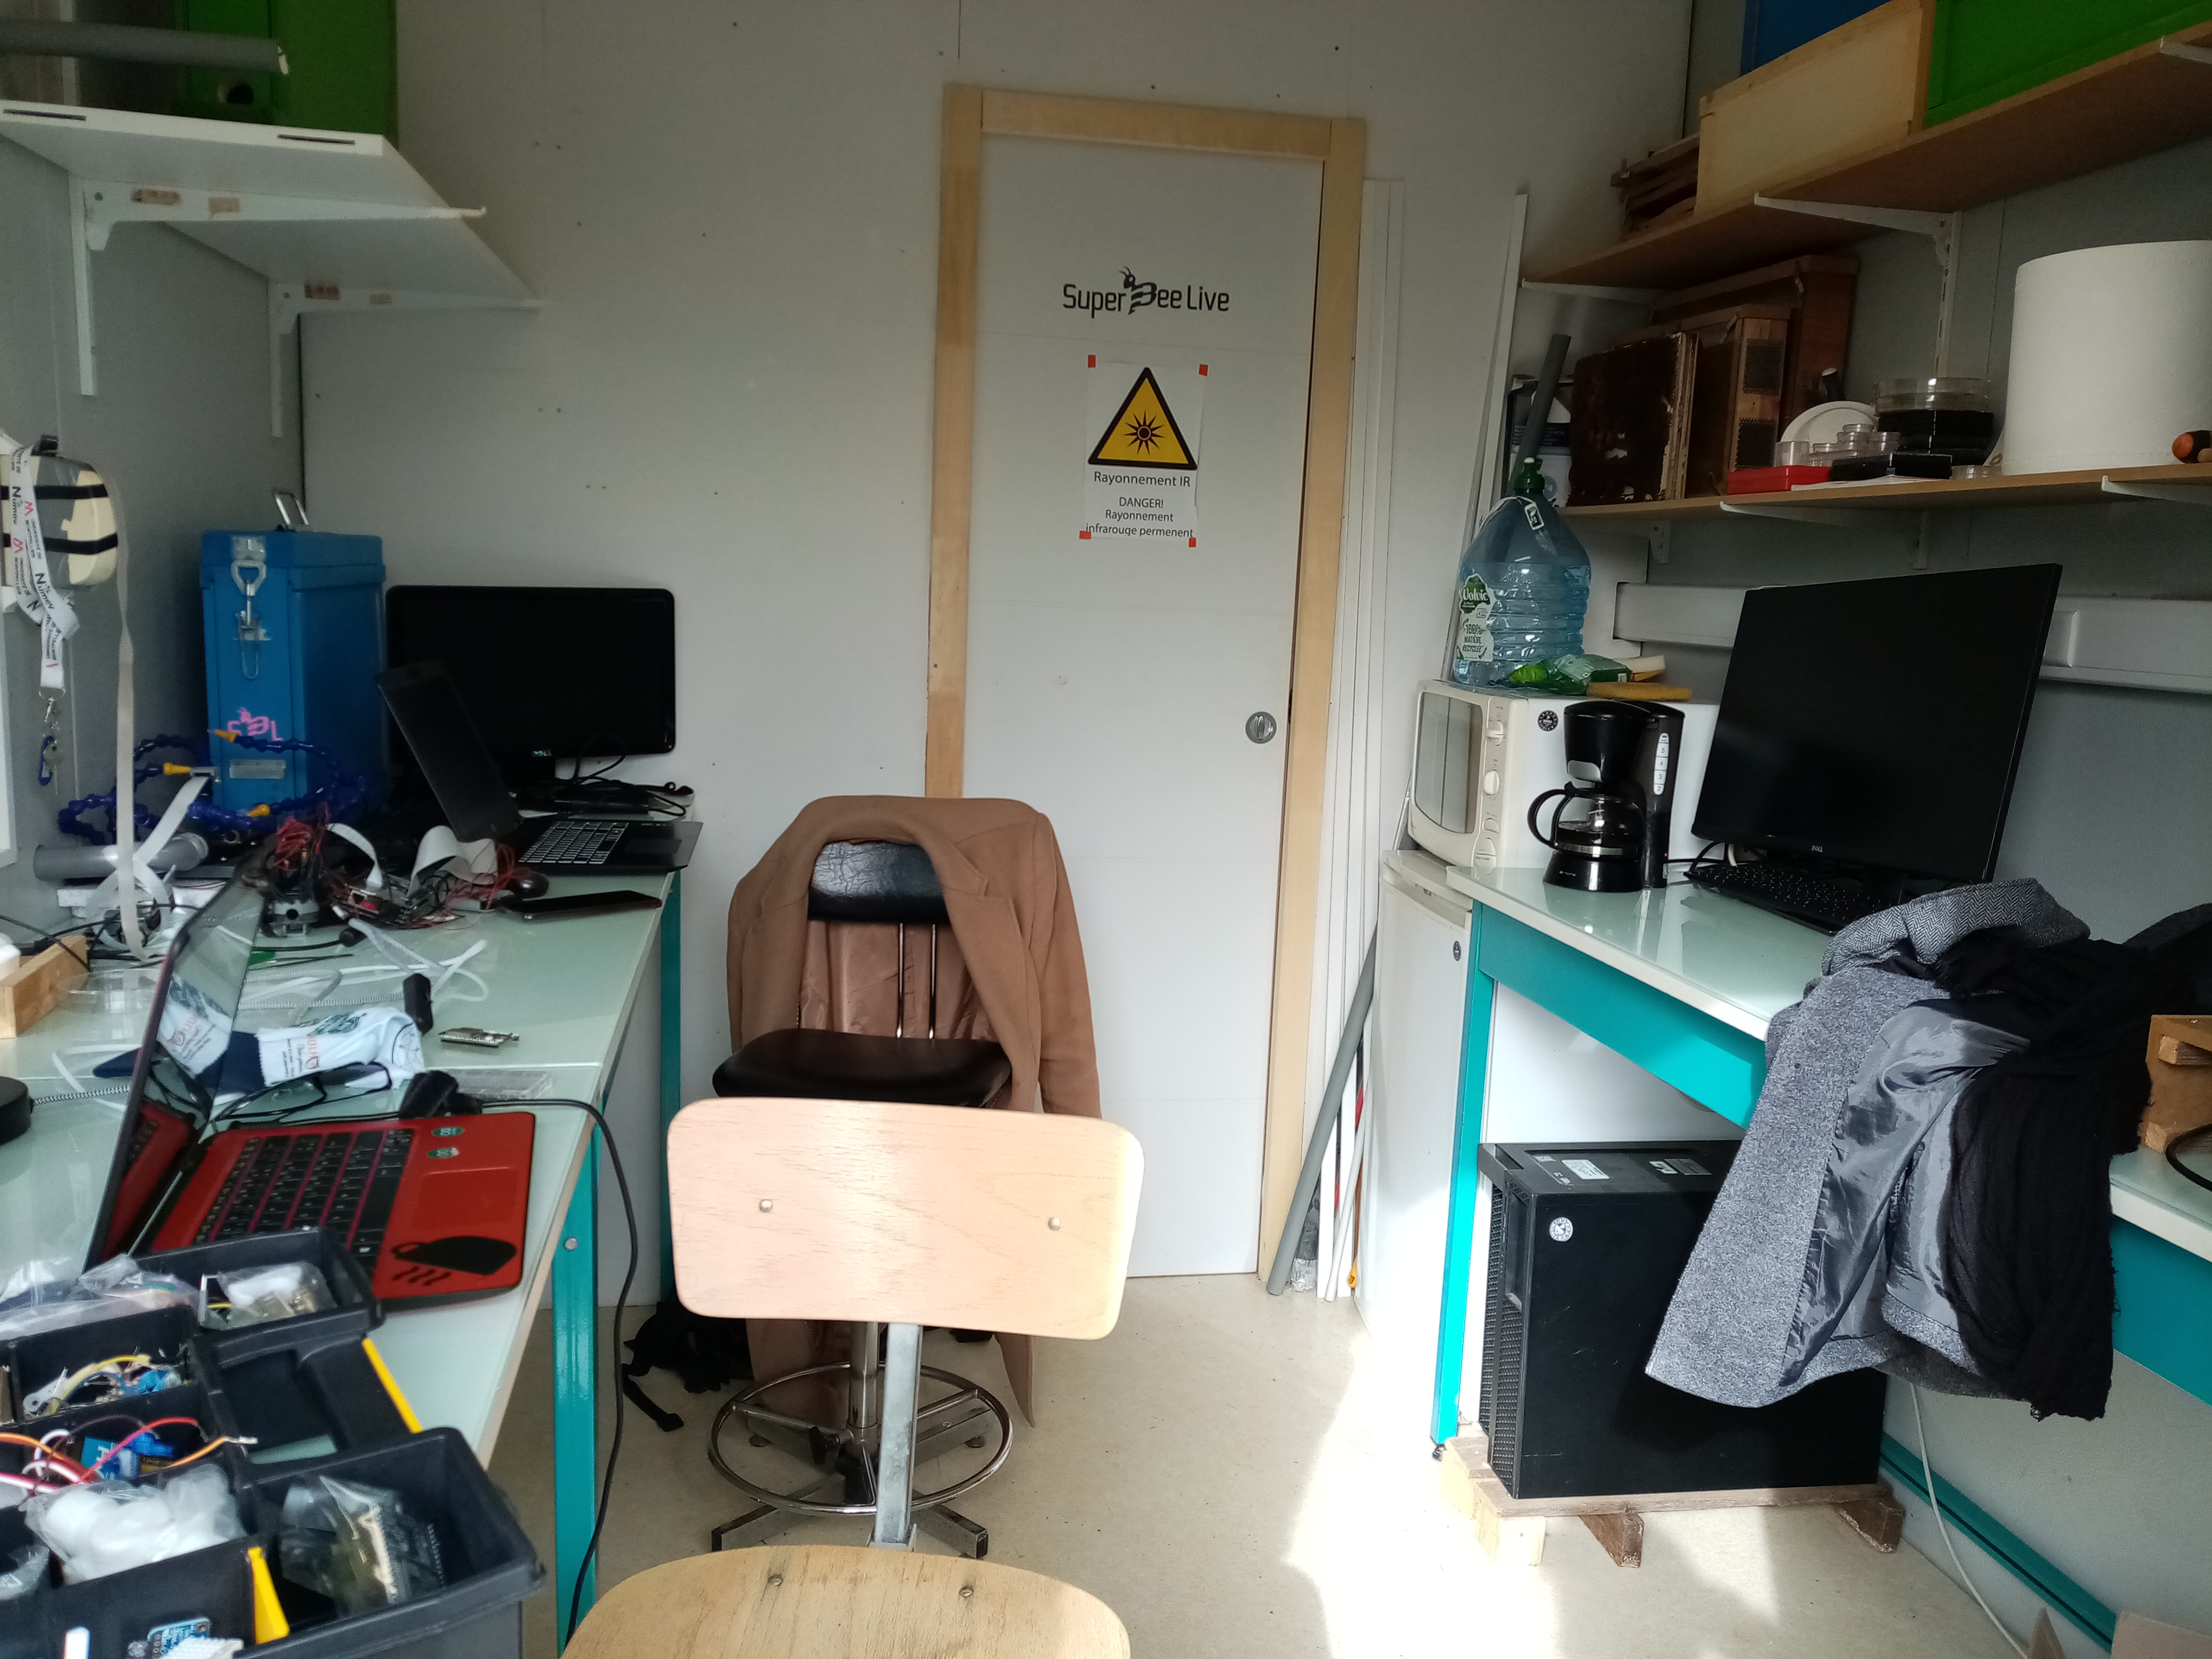
\includegraphics[scale=0.075]{../img/interieur_rucher.jpg}
\captionof{figure}{Intérieur du rucher}
\label{image1}
\includegraphics[scale=0.075]{../img/exterieur_rucher.jpg}
\captionof{figure}{Extérieur du rucher}
\label{image2}
\end{center}


\newpage
\section{Organisation}
\subsection{Notion}
Afin de pouvoir m'organiser et avoir un suivi de mon activité tout au long du stage, j'ai mis en place un Gantt sous la forme d'une page Notion.
Chaque page que j'ai créé sur notion possède une fonction précise. Je vais donc vous présenter brièvement chacune d'entre elles.

\subsubsection{Calendrier}
Comme son nom l'indique, la page calendrier répertorie chaque tâche ayant été effectuée sous la forme d'un calendrier. Celle-ci me permet de m'organiser sur le mois à venir et surtout de garder un oeil sur l'échéances. 
\begin{center}	
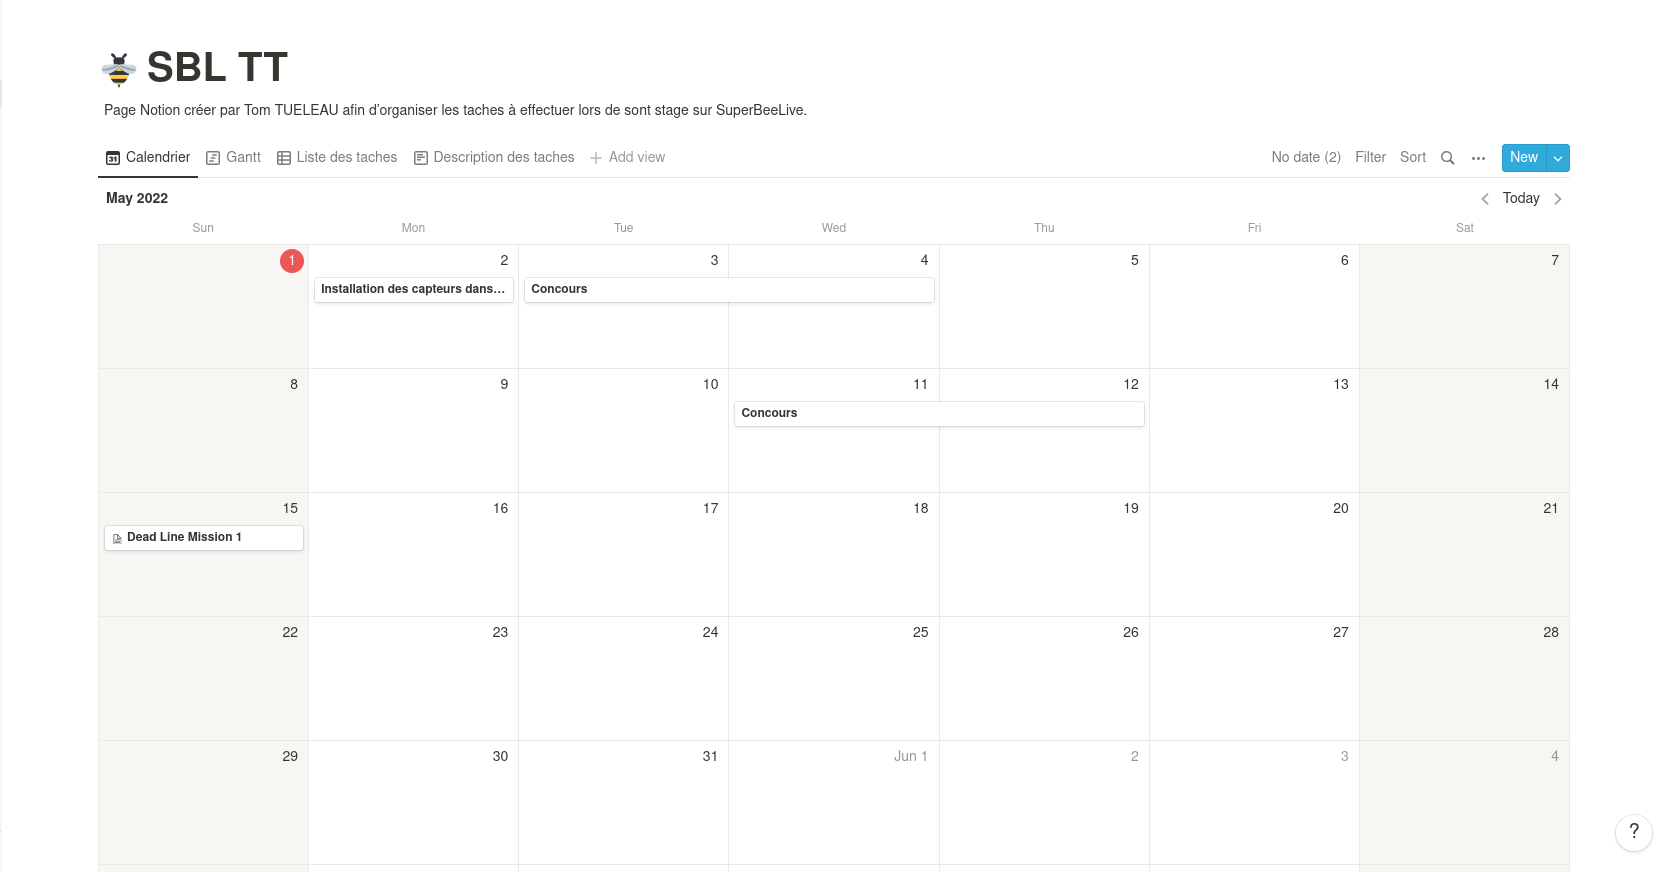
\includegraphics[scale=0.35]{../img/notioncalender.png}
\captionof{figure}{Calendrier}
\label{Calendrier}
\end{center}

\subsubsection{Liste des tâches}
La page liste des tâches regroupe toutes les tâches effectuées et à effectuer. J'attribue à ces tâches des étiquettes ce qui me permet de les classer.   
\begin{center}	
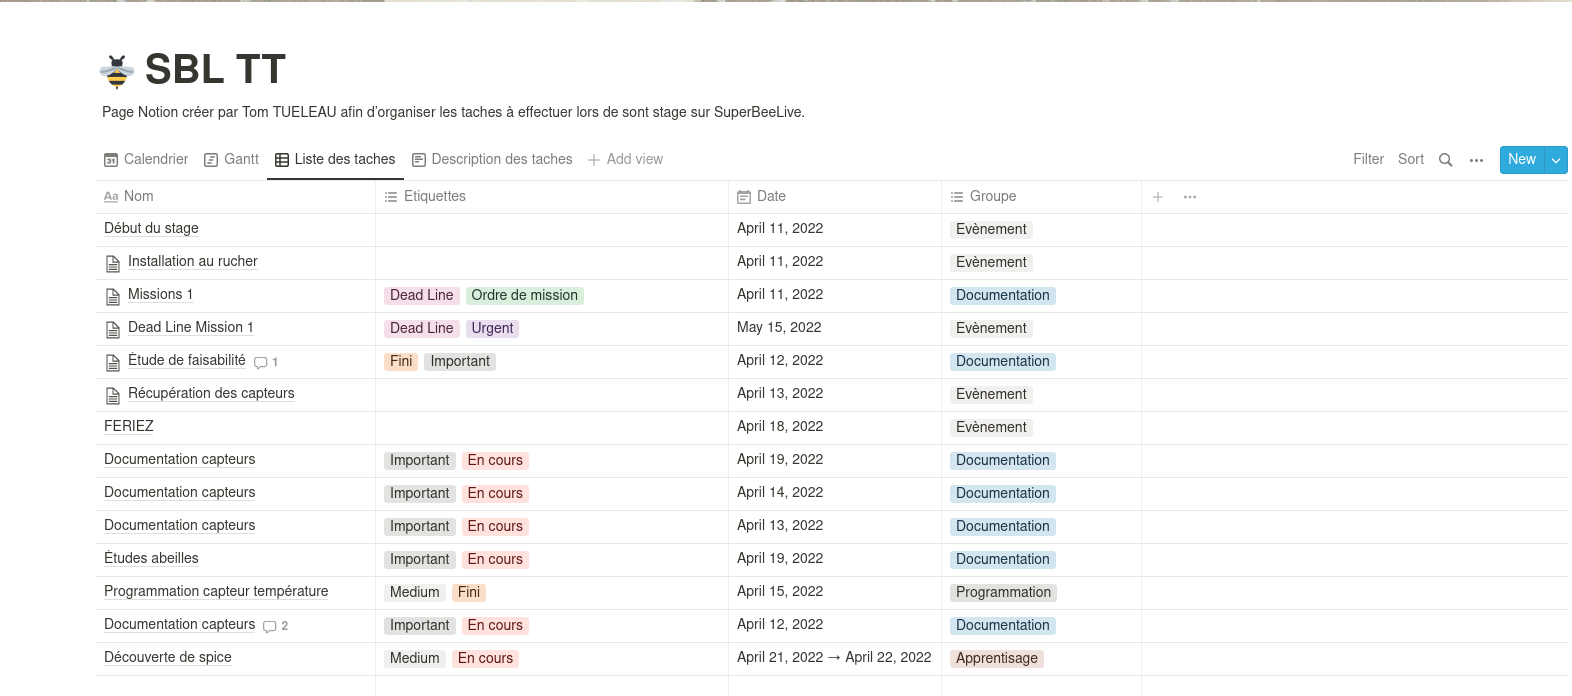
\includegraphics[scale=0.35]{../img/notionlistesdestaches.png}
\captionof{figure}{Liste des tâches}
\label{Liste des taches}
\end{center}

\subsubsection{Description des tâches}
Cet onglet contient une description plus détaillée des tâches. J'y stocke aussi les compte-rendu de réunion, prises de note, images relatives à mes parties du projet.
\begin{center}	
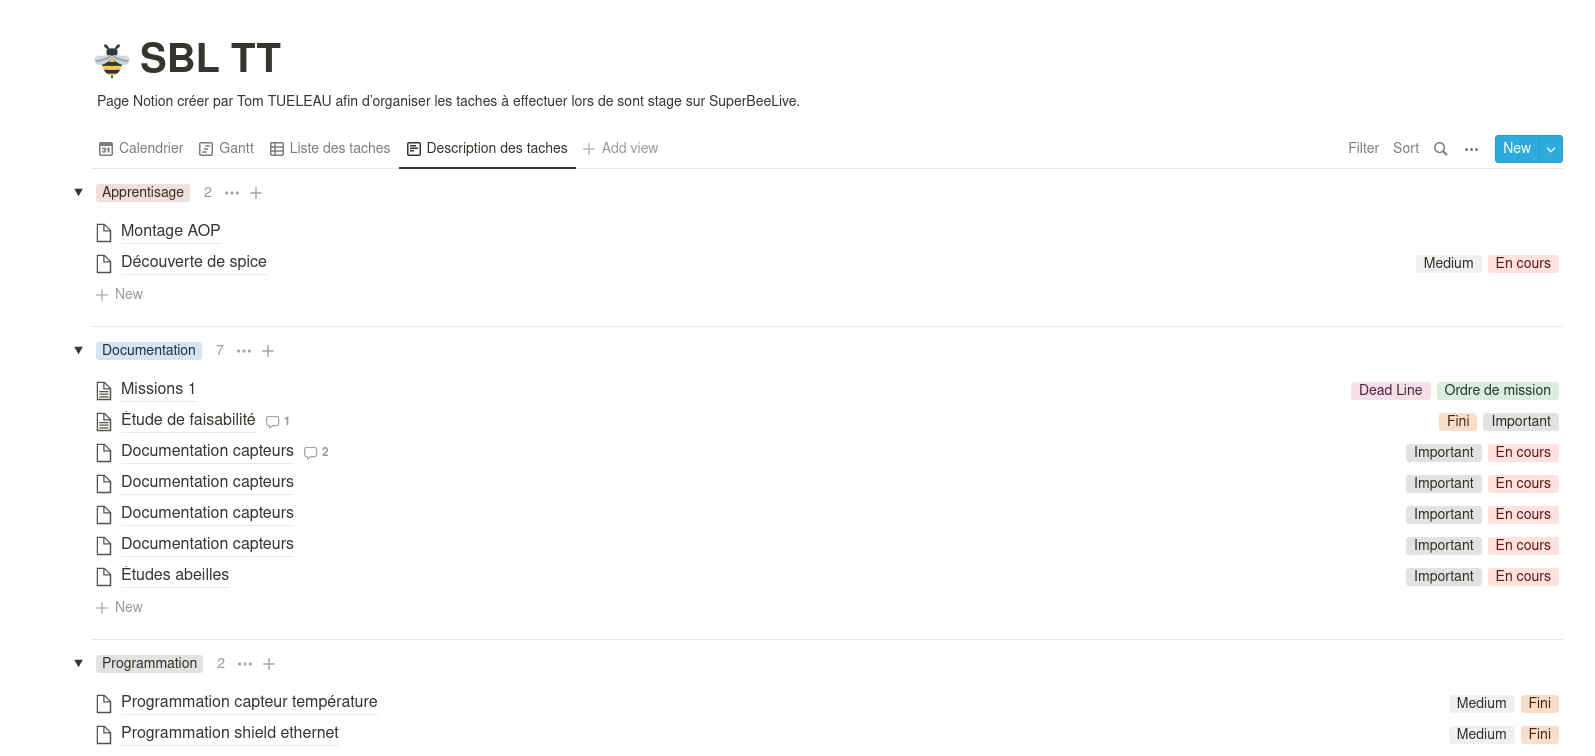
\includegraphics[scale=0.35]{../img/notiondescriptiondestaches.png}
\captionof{figure}{Description des taches}
\label{Description des taches}
\end{center}

\subsubsection{Gantt}
La dernier fiche accessible est la fiche "Gantt" qui me permet surtout de m'organiser sur ma semaine. 
\begin{center}	
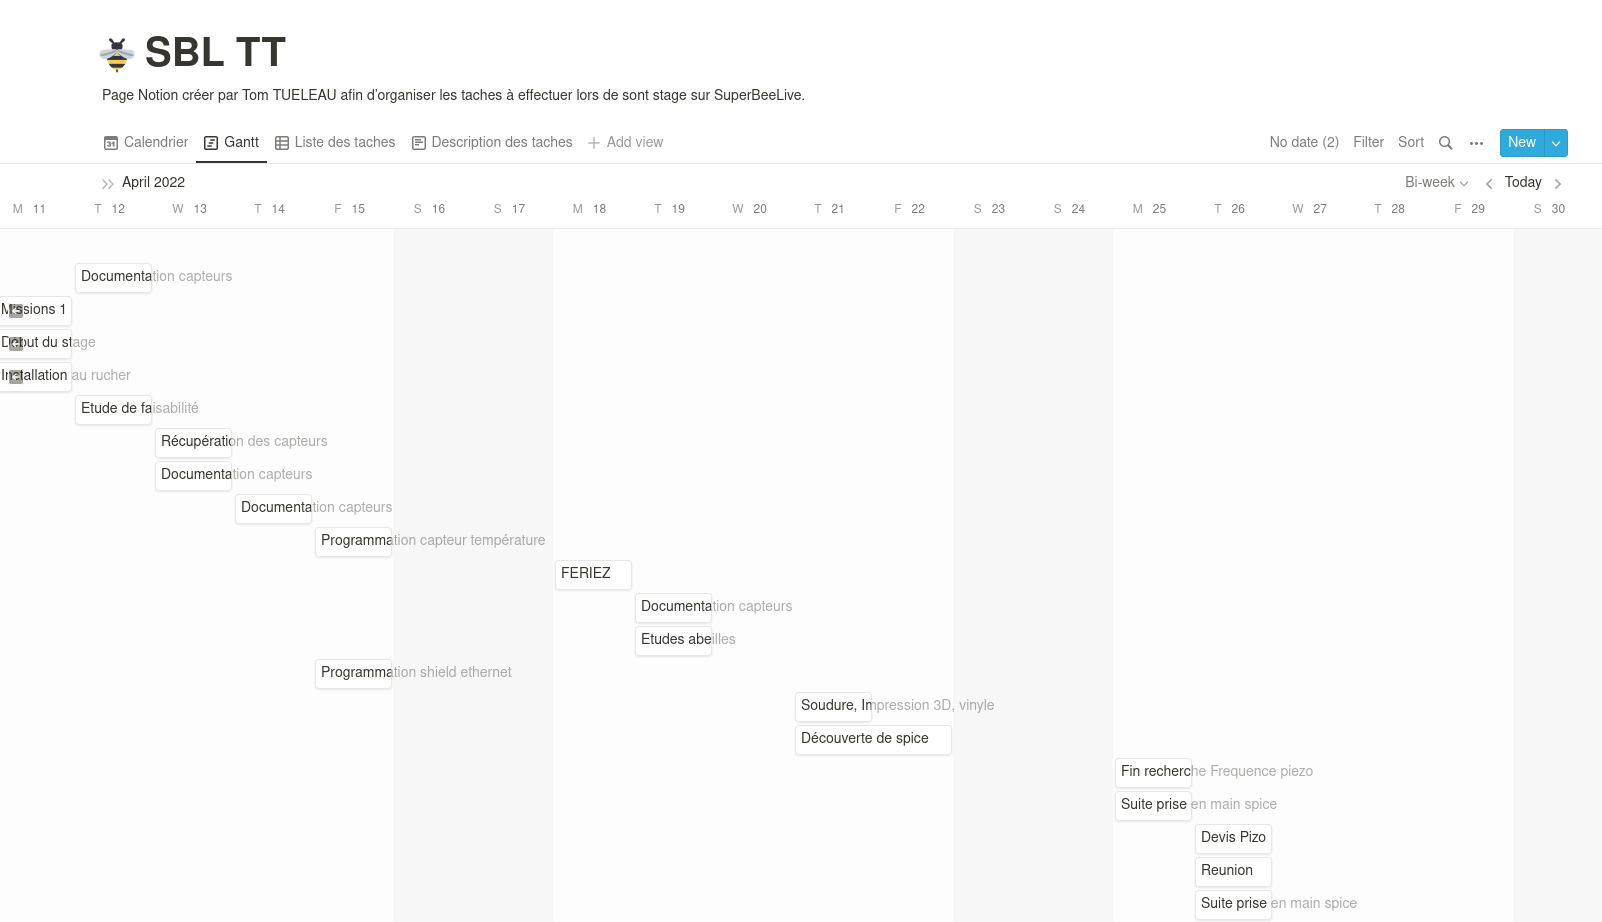
\includegraphics[scale=0.35]{../img/notiongantt.png}
\captionof{figure}{Gantt}
\label{Gantt}
\end{center}
\newpage 

\newpage

\section{Topologie Réseau}
\subsection{Rucher}
\subsection{Serveur}
\subsection{Microcontroleur}

%%%%%%%%%%%%%%%%%%%%%%%%%%%%%%%%%%%%%%%%%%%%%%%%%%%%

%%%%%%%%%%%%%%%%%%%%%%%%%%%%%%%%%%%%%%%%%%%%%%%%%%%%

\newpage
\section{Eléctronique}
\subsection{Choix des composants}

Le but de cette section est d'énoncer les possibilités que j'ai trouvées en ce qui concerne les composants demander (Capteurs d'humiditer de température et de vibration et mico-controleur). Nous commencerons par voir les différentes possibilités pour le micro-contrôleur et le choix effectuer. Ensuite, j'évoquerais les modèles des capteurs d'hygrométrie et de température aux quels j'ai songé. Enfin, je reviendrais sur le cas du capteur de vibration et les probématiques que j'ai pu rencontrer à sont égare.

\subsubsection{Micro-controleur}

Afin de remplire la mission, le micro controleur doit pouvoir :\\
\\
	- Récolter les données des differents capteurs\\
	- Envoyer les données via MQTT\\
	- Mise en place rapide et facile\\
	\\
De ces trois critères, j'ai retenue deux solutions possibles. 
Tout d'abord un arduino muni d'un shield Ethernet pourrait nous permettre dans un premier temps d'avoir un système 
connecté à internet et simple à mettre en place.
Dans un second temps, j'ai pensé à un Esp32 qui permettrait de faire transiter les données en Wifi et qui est plus petit. 
Étant familiarisé avec les deux solutions je n'avais pas de préférence. J'ai cependant commencé à travailler sur l'arduino, car j'avais
le matériel à disposition.

\subsubsection{Capteur de température et d'hygrométrie }
Pour répondre à ce besoin, j'ai opté pour un Si7021. J'ai fait ce choix, car le capteur était directement à disposition et que je l'avais déjà programmé. Leurs caractéristiques sont les suivantes :\\
\\
Température :\\
\begin{center}
    \begin{tabular}{|l|l|}
	\hline
	    Plage de valeur & Résolution \\
	\hline
	    -40C - 125C & 0,4C \\
	\hline
    \end{tabular}
\end{center}
Humidité:\\
\begin{center}
    \begin{tabular}{|l|l|}
	\hline
	    Plage de valeur & Résolution \\
	\hline
	    0\% - 80\% & 0,3\% \\
	\hline
    \end{tabular}
\end{center}

\subsubsection{Capteur de vibration}
Le capteur de vibration est la partie que je connais le moins du projet. J'ai pu trouvé deux solutions.\\
 Une première à l'aide d'un capteur piézo-électrique et une seconde avec un  microphone. Ces deux capteurs étant les seules possibilités que j'avais à ma disposition, 
 j'ai décidé de les tester afin de savoir si elles pouvaient répondre aux besoins du projet.\\
\\
 Les deux références sont :\\
- p37e pour le piézo-électrique\\
- INMP441 pour le microphone.\\

\subsection{Montages AOP}

Lors de ce stage j'ai du faire des recherches quand au dimensionnement d'un montage amplificateur. Ce besoin s'était fait ressentir quand je m'étais rendu compte que le signal émis par le piézo-électrique n'arrivait pas à être capté par l'Arduino.  Dans cette partie nous verrons tout d'abord le cheminement effectuer afin d'obtenire un montage fonctionnel. 

\subsubsection{Amplificateur de mesure}

Lors de cette semaine je suis donc passé au montage amplificateur de mesure. Ce montage est très souvent utilisé afin d’amplifier le signal de sortie d’un capteur ayant une tension trop faible.
Il existe plusieurs montages amplificateur de mesures. Dans mon cas, j’ai commencé par un montage nécessitant 3 AOP. Nous pouvons voir ce montage figure \ref{3AOP}

\begin{center}	
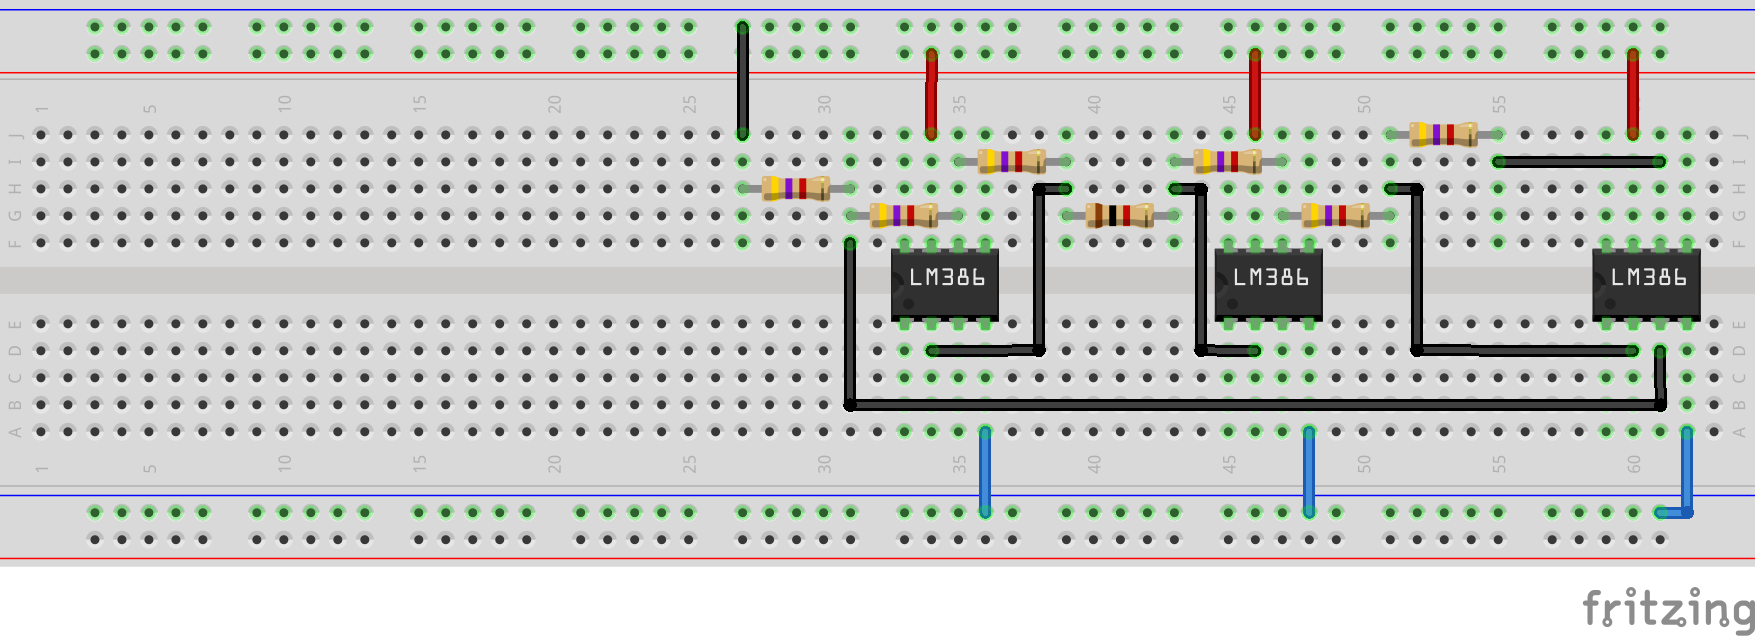
\includegraphics[scale=1]{../img/instrumentation3aop_bb.png}
\captionof{figure}{Montage 3 AOP sous Fritzing}
\label{3AOP}
\end{center}


Il existe cependant des montages plus simples notamment un composé de deux amplificateurs opérationnels que l'on peut voir figure \ref{2AOP}.
\\

\begin{center}	
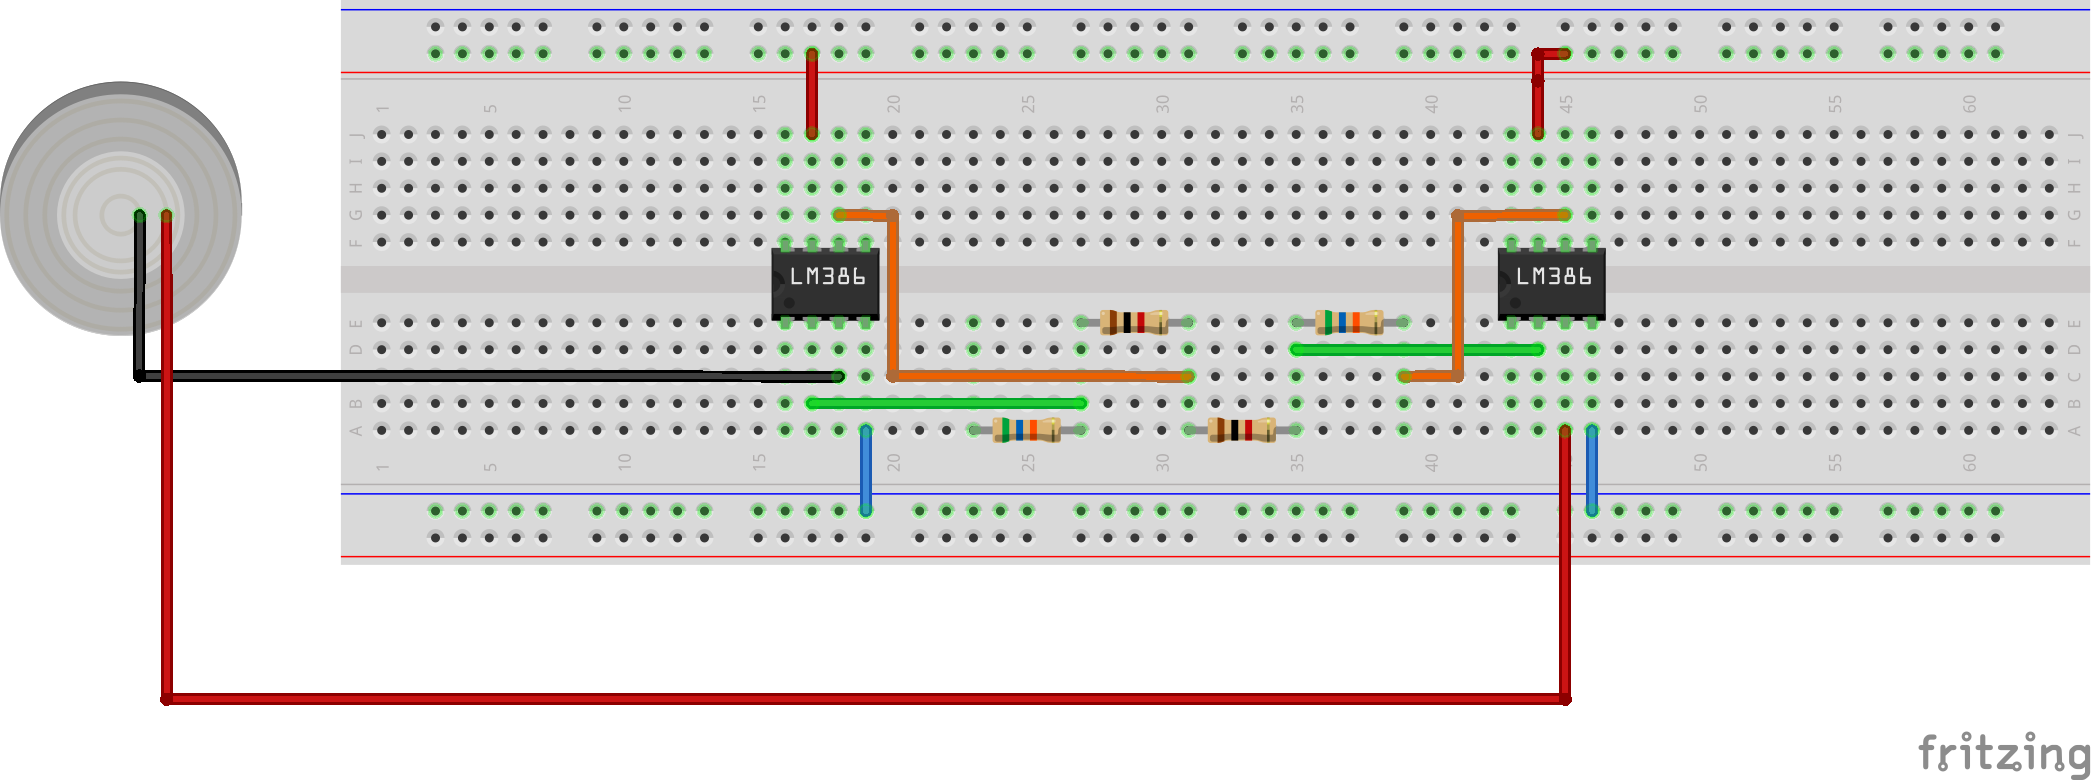
\includegraphics[scale=0.80]{../img/instrumentation2aop_bb.png}
\captionof{figure}{Montage 2 AOP sous Fritzing}
\label{2AOP}
\end{center}

Aprés avoir réussi à effectuer ce montage, j’ai pu remarquer que la sensibilité avait diminué. Ceci a eu pour effet de d’empêcher la visualisation de l’impulsion créée lors de petits frottements. Après plusieurs tentatives de modification pour pallier à ce changement, j’ai décidé de changer de montage.

\subsubsection{Montage actuel}
Le piezo-electrique utilisé jusqu’à maintenant était fourni avec un module. Celui-ci ne changeait rien au signal et pour cause, les composants sur lui n’étaient pas totalement connectés. Cependant, après avoir effectué des modifications sur celui-ci le signal m'a paru beaucoup plus net.
J’ai par la suite effecuté le montage visible figure \ref{MTGFINAL}
\\
\begin{center}	
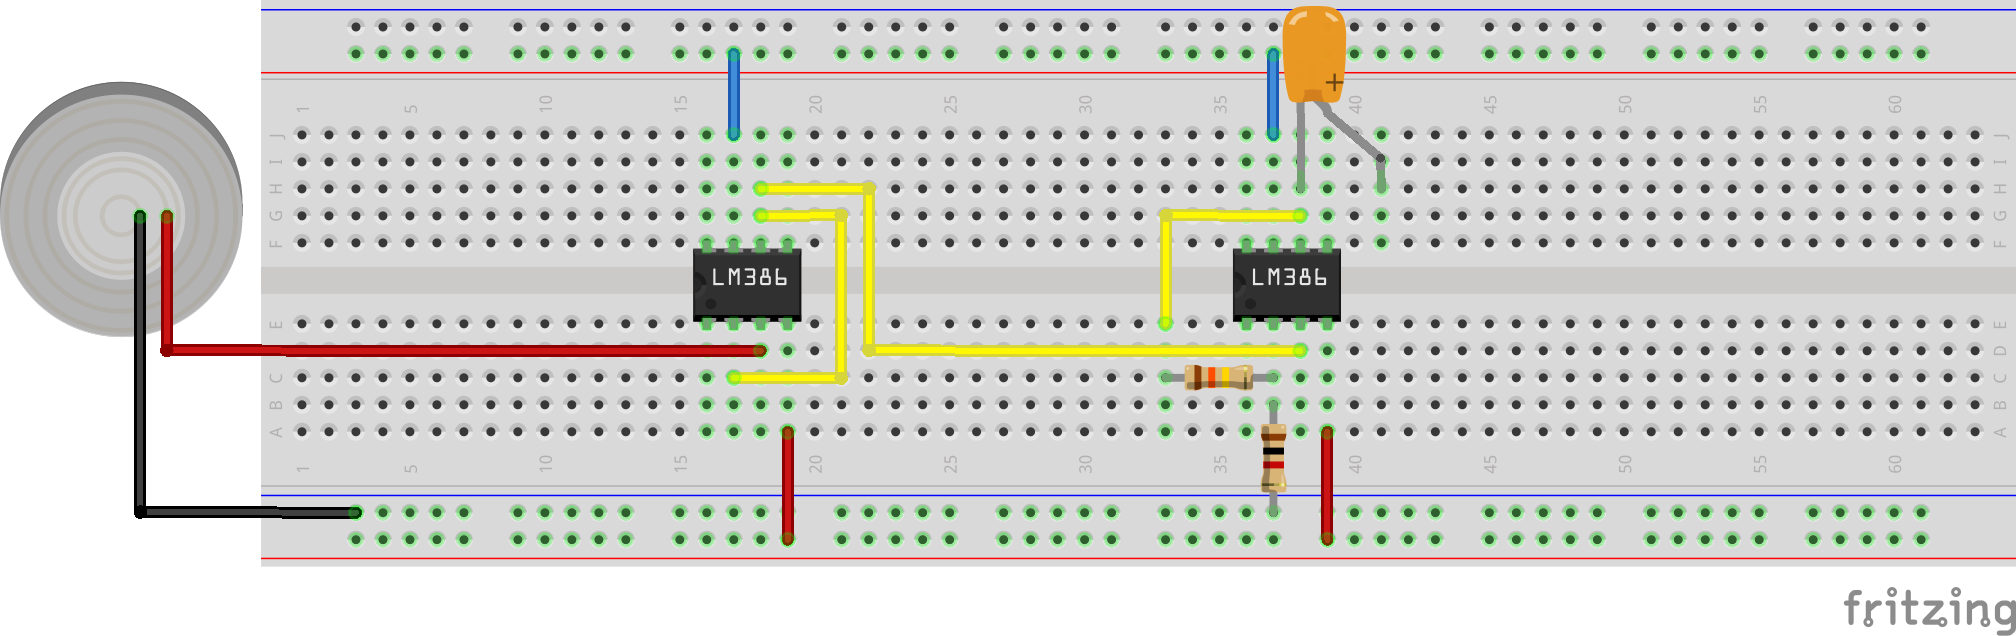
\includegraphics[scale=0.85]{../img/mtgfinal.png}
\captionof{figure}{Dernier montage }
\label{MTGFINAL}
\end{center}
Il est composé d’un suiveur et d’un amplificateur non-inverseur avec un coefficient multiplicateur de 130. C'est à dire que la tension de sortie sera 130 fois la tension d'entrée. Enfin, un condensateur se trouvant en sortie de circuit nous permet d’éliminer la composante continue ajoutée par les AOP à notre signal.


\subsubsection{Résultat}
Avec le montage vue précédemment nous obtenons plusieurs résultats probants.
Tout d'abord, nous pouvons voir figure \ref{VWOMVM} le signal en sortie du montage quand aucun évènement ne se produit.
Ensuite figure \ref{F}, nous pouvons voir la réaction après un léger frottement effectué avec un câble visible figure \ref{M}. 

\begin{center}	
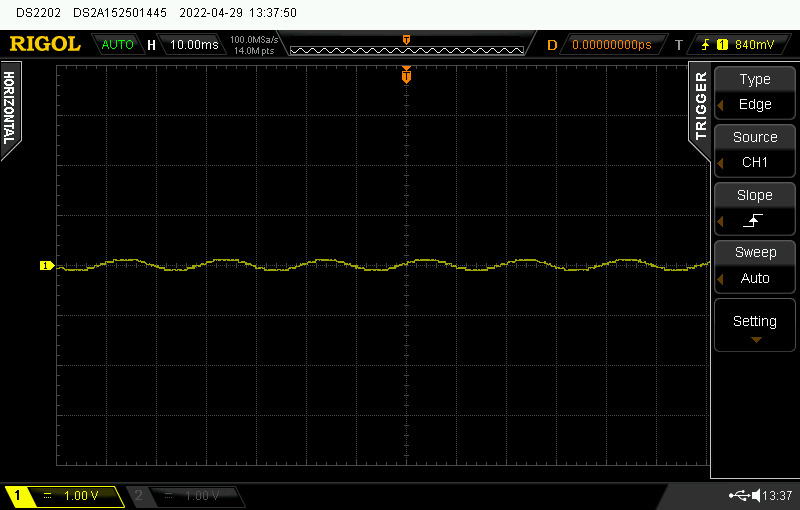
\includegraphics[scale=0.5]{../img/plat.jpg}
\captionof{figure}{Tension sans mouvement}
\label{VWOMVM}
\end{center}

\begin{center}	
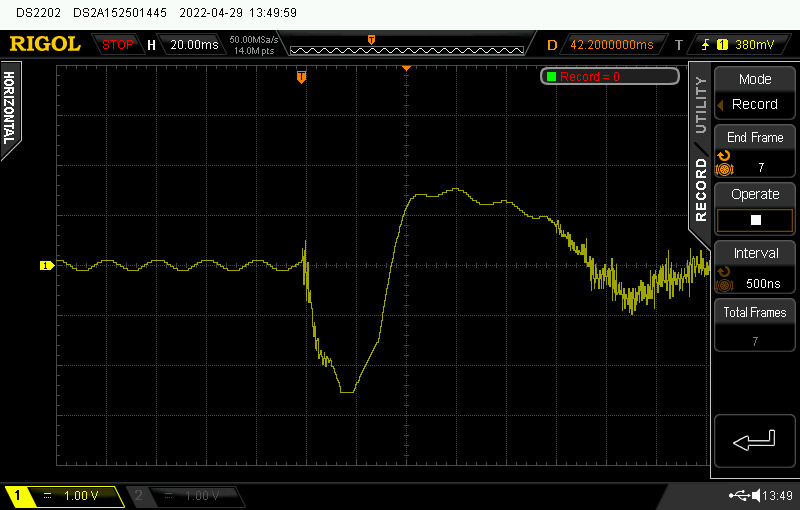
\includegraphics[scale=0.5]{../img/frotment.jpg}
\captionof{figure}{Tension lors d'un Frottement}
\label{F}
\end{center}

\begin{center}	
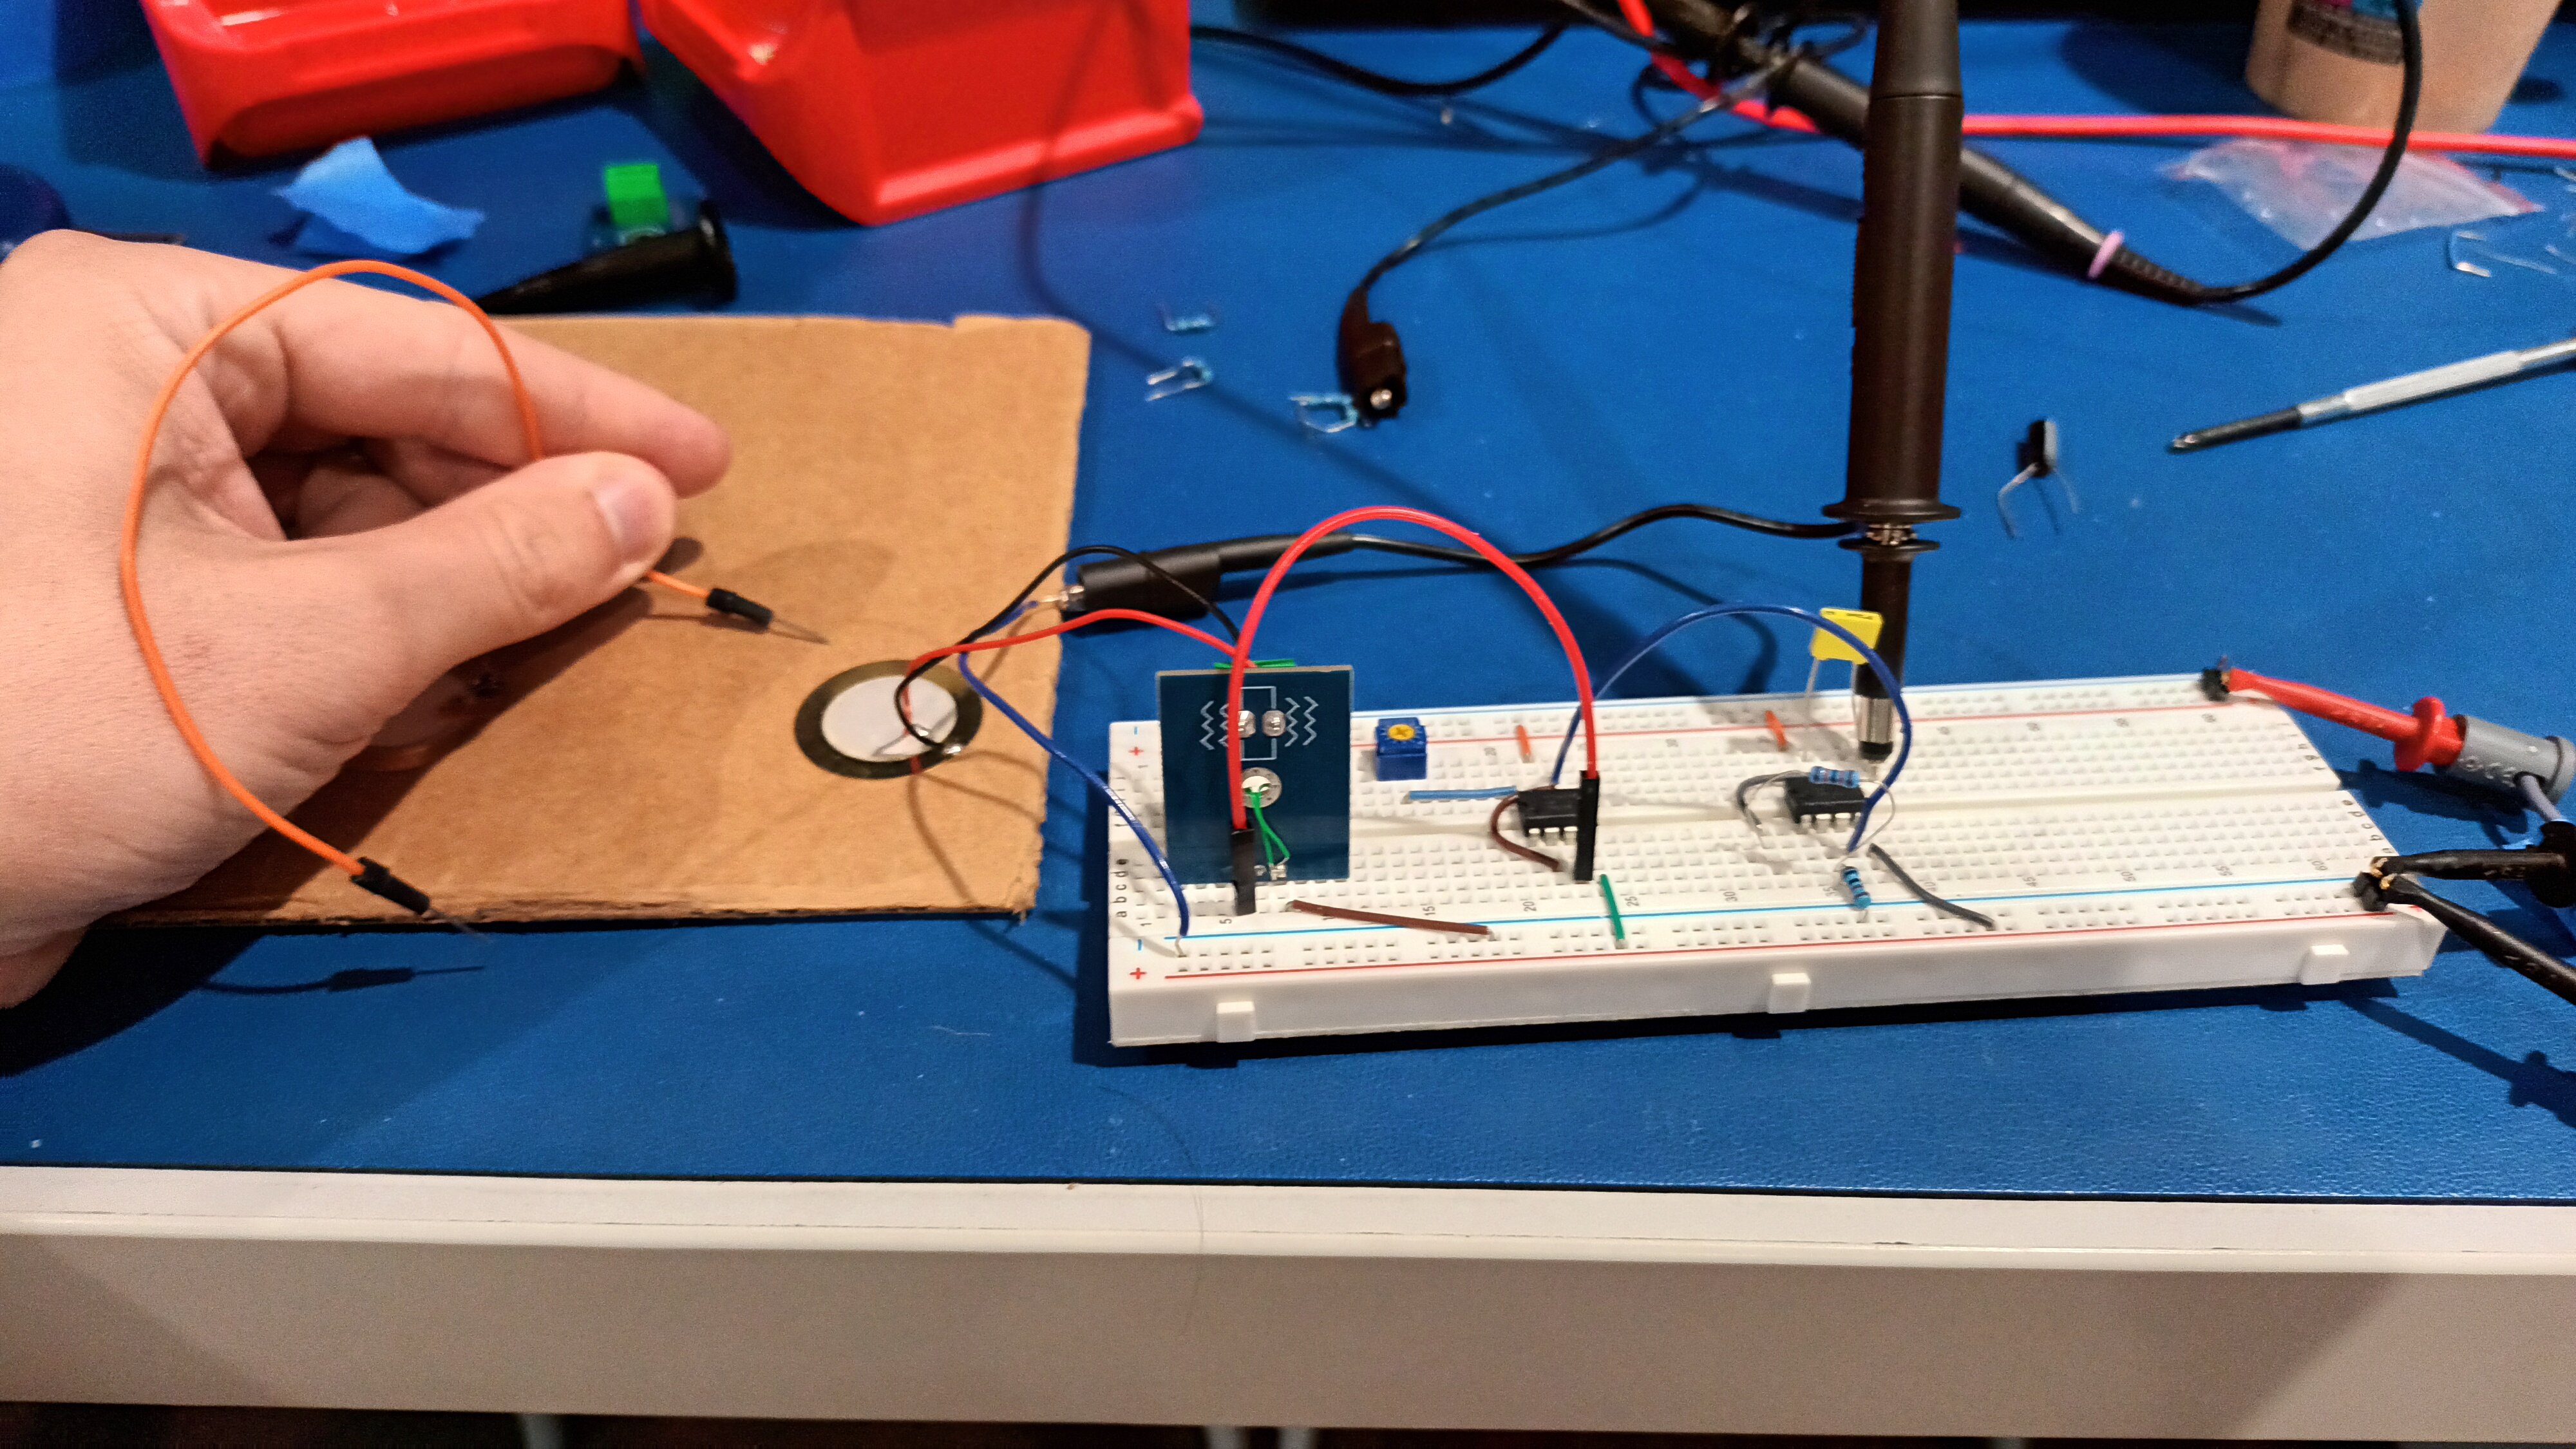
\includegraphics[scale=0.1]{../img/froty.jpg}
\captionof{figure}{Frottement}
\label{M}
\end{center}
\subsection{PCB}

\newpage
\section{Programmation}
\subsection{Réseau}
\subsection{Capteurs}

%%%%%%%%%%%%%%%%%%%%%%%%%%%%%%%%%%%%%%%%%%%%%%%%%%%%

%%%%%%%%%%%%%%%%%%%%%%%%%%%%%%%%%%%%%%%%%%%%%%%%%%%%
\newpage
\section{Conclusion}
En conclusion, ce stage à été formateur pour moi tant dans l'approche que j'ai du mettre en place pour solutionner les probléme possé, que dans les différents domaines aborder. J'ai cependant rencontrer des difficulter sur certaine partie. En effet mes compétence en éléctronique ce limitant à des basique, j'ai abordées des composants complex comme l'amplificateur-opérationel avec certaine difficulter. J'ai cependant pu conter sur l'aide de mes encadrants afin de me diriger vers les bonnes sources d'information.


\newpage
\listoffigures

\newpage
\section*{Annexe}
\subsection*{Code}
\subsection*{Fichier de configuration}

\end{document}
